\chapter{Theory}
%\subsection{Introduction to Mixing Phenomenology}
\section{Review of the Standard Model}
The Standard Model (SM) of particle physics is to-the-date the most accurate model describing the buildings blocks of matter (particles) and their interactions (via forces). In particular SM describes all the fundamental forces but gravity: electromagnetic, strong nuclear, and weak nuclear force. It is a quantum field theory (QFT), whereby the dynamics of the system is captured by the most general renormalisable Lagrangian density that is invariant under gauge symmetry. QFT considers particles to be an excited states of an underlying field, also known as quanta. In the SM particles and forces are the results of interactions between scalar, vector and spinor fields. In general there are two sets of particles: force-carrying particles also known as bosons, which have integer spin and are quanta of the scalar and vector fields. More specifically, there is thes Higgs boson, the only elementary scalar boson in the SM, and vector bosons: gluons, $W^{\pm}$, Z and $\gamma$. Secondly, there are the non-force carrying particles, which are known to be fermions, quanta of spinor fields. Unlike bosons they carry half-integer spin. These can be further classified into two elementary families of particles: quarks, which cannot be observed alone and leptons which can be detected on their own. Out of all of these fundamental particles, those that have mass acquire it by the most famous symmetry-breaking mechanism - Higg's mechanism.

Quarks are affected by all three fundamental forces. They come in six different \textit{flavours} and they carry fractional charge as seen in~\autoref{nonlin}.

\begin{table} 

\centering % used for centering table 
\begin{tabular}{|c|c|c|c|} % centered columns (4 columns) 
\hline %inserts double horizontal lines 
Generation & ``Flavour" & Charge & Constituent Mass \\ [0.5ex]\hline% inserts table 
%heading 
\hline % inserts single horizontal line 
1st & up  \textit{u}& +2/3 & ~300 Mev/c$^{2}$ \\ % inserting body of the table 
1st & down \textit{d}& -1/3 &  ~300 MeV/c$^{2}$ \\[1ex]
2nd & charm \textit{c}& +2/3 &  ~1.5 Gev/c$^{2}$\\ 
2nd & strange \textit{s}& -1/3 &  ~500 Mev/c$^{2}$ \\[1ex]
3rd & top \textit{t}& +2/3 &  ~175 Gev/c$^{2}$ \\ 
3rd & bottom \textit{b}& -1/3 & ~ 5 Gev/c$^{2}$ \\ [1ex] % [1ex] adds vertical space 
\hline %inserts single line 

\end{tabular} 
\caption{Quarks and their properties.} 
\label{nonlin} % is used to refer this table in the text 
\end{table} 

The reason why quarks are not observed alone is due to their confinment within hadrons, which is an artefact of strong interaction acting on quarks. This can be understood within the framework of quantum field theory by observing evolution of the coupling strenght $g$ as a function of energy scale, also known as $\beta$ function.
The $\beta$-function for a coupling constant $g$ in the SM to the two loop contribution takes the following form:
\begin{equation}
\beta_g = \mu {{d g}\over d \mu} = {1\over16\pi^2} \beta_g^{(1)}
+ {1\over(16\pi^2)^2} \beta_g^{(2)},
\end{equation}
where $\beta_g^{(1)},~ \beta_g^{(2)}$ denote the one-loop and two-loop
contributions respectively, and $\mu$ is the energy scale. For the strong interaction, unlike electromagnetic and weak interaction, $\beta_g$ is negative. For low energies as $\mu \rightarrow 0$ the coupling is very high and hence quarks cannot be observed on their own, \textit{confinement}. On the other hand as $\mu \rightarrow \infty$, or at high energies, the coupling gets small, particles get decoupled, which is known as \textit{asymptotic freedom}. 

There are altogether 12 leptons. Unlike quarks they are not affected by strong force but also come along in three generations: electrons, muons and taus. They have their equivalent antiparticles and corresponding neutrinos. Much of this thesis is dedicated to the study of the muons, antimuons and their neutrinos with LHCb detector.


\section{Principle of Standard Model Building}
In more mathematical terminology, the SM is a theory that respects SU(3)$\otimes$SU(2)$\otimes$U(1) symmetries. In this section the form of the Lagrangian density of the SM is motivated. It is assumed that $\hbar=1$, $c=1$. Let $\psi$ to be a spinor field. The Dirac Lagrangian for spin-$\frac{1}{2}$ non-interacting or free field for a particle with mass $m$ can be written as: 
\begin{equation}
\mathcal{L} = i\overline{\psi}\gamma^{\mu}\partial_{\mu}\psi - m\overline{\psi}\psi.
\label{eq:lag_first}
\end{equation}

where $\gamma^{\mu}$ are $4\times 4$ Dirac matrices and $\mu\in\{0,1,2,3\}$.

By using Euler-Lagrange equation in the relativistic theory

\begin{equation}
	\partial_{\mu}\Big(\frac{\partial{\mathcal{L}}}{\partial(\partial_{\mu}\psi_{i})} \Big) =\frac{\partial \mathcal{L}}{\partial\psi_{i}}
\label{eq:lag_first}
\end{equation}

for $\overline\psi$ the Dirac equation of motion

\begin{equation}
 i\gamma^{\mu}\partial_{\mu}\psi - m\psi = 0
\label{eq:lag_first}
\end{equation}

is retrieved.

The Dirac Lagrangian in~\autoref{eq:lag_first} stays the same under global phase transformation: $\psi \rightarrow e^{i\phi}\psi$ as $\overline\psi \rightarrow e^{-i\phi}\overline\psi$. However, undel local phase transformation, where $\phi$ is a function of $x^{\mu}$  this is not the case anymore. In this case
\begin{equation}
\mathcal{L} \rightarrow \mathcal{L}- (\partial_{\mu}\phi) \overline{\psi}\gamma^{\mu}\psi.
\label{eq:notinv}
\end{equation}

By requiring local gauge invariance for the Lagrangian, it is necessary to add a term to counteract the left-over term in~\autoref{eq:notinv}. Let $\lambda=-\frac{\phi(x)}{q}$ and let $A_{\mu}$ be some new (vector) field which transforms as $A_{\mu} \rightarrow \partial_{\mu}\lambda$ then the following Lagrangian

\begin{equation}
	\mathcal{L} = i\overline{\psi}\gamma^{\mu}\partial_{\mu}\psi - m\overline{\psi}\psi - q\overline{\psi}\gamma^{\mu}\psi A_{\mu}
\label{eq:lag_sec}
\end{equation}

stays invariant under local phase transformation. That is good, however, there is a penalty for introducing a new vector field $A_{\mu}$ which interacts with spinor field $\psi$ as can be seen in the last part of~\autoref{eq:lag_sec}, that is a non-interacting term for $A_{\mu}$.

The Lagrangian for non-interacting vector field for a particle with mass $m_{A}$ with the field strenght $F^{\mu\nu}=\partial^{u}A^{\nu} - \partial^{\nu}A^{u}$ is
\begin{equation}
\mathcal{L}= -\frac{1}{16\pi} F^{\mu\nu}F_{\mu\nu} + \frac{1}{8\pi}m_{A}^{2}A^{\mu}A_{\mu}.
\end{equation}

In order not to spoil the local gauge invariance the $m_{A}=0$. Hence the full Dirac Lagrangian with local phase invariance introduces massless vector field $A^{\mu}$ yields

\begin{equation}
	\mathcal{L} = i\overline{\psi}\gamma^{\mu}\partial_{\mu}\psi - m\overline{\psi}\psi - q\overline{\psi}\gamma^{\mu}\psi A_{\mu} -\frac{1}{16\pi} F^{\mu\nu}F_{\mu\nu},
\label{eq:lag_thir}
\end{equation}

which can be recognized as the Lagrangian for quantum electrodynamics (QED), whereby the electrons and positrons (quanta of spinor field) are interacting with photons (quanta of vector field). In other words, $A_{\mu}$ is electromagnetic potential and $q=e$, the current density is hence $J^{\mu}=e\overline{\psi}\gamma^{\mu}\psi$. This represents U(1)  

To upgrade from global invariance of the non-interacting Lagrangian in~\autoref{eq:lag_first} to local invariance one can also achieve it in one step be defining \textit{covariant derivative}
\begin{equation}
	\mathcal{D}_{\mu} = \partial_{\mu}+ iqA_{\mu},
\end{equation}

where the secret ingredient is to transform the partial derivative in the same way as the field itself undel local gauge transformation.

\section{Quantum Chromodynamics}
Requirement of gauge invariance under local transformation is a powerful tool and it is used throughout the Standard Model building. In this section the development of Lagrangian for Quantum chromodynamics (QCD) is explained. QCD dectribes strong interactions or nuclear binding forces and makes use of quarks ($q$) whereby most of the time they are observed to be bound either in pairs - mesons ($q\bar{q}$) - or triplets - baryons ($qqq$). The interactions between quarks and gluons are described by $SU(3)_{C}$ gauge group. The conserving charge associated with strong force is known as color, hence the subpscipt $C$. It was experimentally established that there are 3 colors and borrowing from color theory used by painters these colors are red, blue and green. The quark carries color and antiquark anticolor making mesons and baryons to have zero net color. There are 8 quanta of strong interactions known as gluons.

With these constraints and by requiring the free Lagrangian to be invariant under local $SU(3)$ transformation similarly to the QED case, one obtaines again \textit{covariant derivative}

\begin{equation}
\mathcal{D}_{\mu} = \partial_{\mu} - ig_{s}\frac{\lambda^{a}}{2}G^{a}_{\mu},
\end{equation}

that respects $SU(3)$ symmetry, where $\lambda^{a}$ are Gell-Mann matrices, $a\in\{1..8\}$ (8 possible gluons), $g_{s}$ is the strong coupling. The field strenght for the gluon field is defined as $G_{a}^{\mu\nu}=\partial^{u}G_{a}^{\nu} - \partial^{\nu}G_{a}^{u} + g_{s}f^{abc}G_{b}^{\mu}G_{c}^{\nu}$, where $f^{abc}$ are so-called structure constants which satisfy the following commutaion relation:

\begin{equation}
	\Big[\frac{\lambda^{a}}{2},\frac{\lambda^{b}}{2}\Big] = if^{abc}\frac{\lambda^{c}}{2}.
\end{equation}

As compared to QED field strenght, there is an additional term involving gluon fields themselves, causing cubic and quartic gluon interactions, which were not present before.


Then the full Lagrangian density for the strong interaction then reads as:

\begin{equation}
	\mathcal{L}_{QCD} = i\overline{\psi}\gamma^{\mu}\partial_{\mu}\psi - m\overline{\psi}\psi + g_{s}\overline{\psi}\gamma^{\mu}\frac{\lambda_{a}}{2}\psi G^{a}_{\mu} -\frac{1}{4} G_{a}^{\mu\nu}G^{a}_{\mu\nu},
\label{eq:lag_fourth}
\end{equation}

where the interaction between quarks and gluons is encoded in the third term of~\autoref{eq:lag_fourth}.


\section{Electroweak unification}
The idea behind unification of weak and electromagnetic interactions is very powerful, as it has to accomodate for forces that act with very different strenght with force-carrying particles that are both massive ($W^{\pm}$,$Z$) and masless ($\gamma$). Furthermore $W^{\pm}$ only couple to left-handed particles, whereas, known as parity violation, whereas $Z^{0}$ couple to both left and right-handed particles  electromagnetic vertex factor is purely vectorial($\gamma^{\mu}$) whereas $W^{\pm}$ coupling has both axial and vector components: ($\gamma^{\mu}(1-\gamma^{5})$), where $\gamma^{5}=i\times\gamma^{0}\times\gamma^{1}\times\gamma^{2}\times\gamma^{3}$, which can be solved by absorption of $1-\gamma^{5}$ into a spinor field itself.

In this way one can decompose the spinor field into left-handed and right-handed (chiral) spinors
\begin{equation}
	\psi=\psi_{L}+\psi_{R} = P_{L}\psi + P_{R}\psi
\end{equation}

where $P_{L} =\frac{1-\gamma^{5}}{2}$ and $P_{R}=\frac{1-\gamma^{5}}{2}$ are known to be projection operators. By calling these operators left-handed and right-handed, there is a misconception that $\psi_{L}$ is a helicity eigenstate, but this is only true given the particle in question is masless. These spinors are known to have chirality - known as left or right-handedness. Helicity is rather a projection of the spin on the direction of the momentum.

As the quarks and leptons can couple within the generation exchanging $W^{\pm}$ this gives rise to left-handed isospin doublets and right-handed isospin singlets. The simplest group with doublet representation is SU(2) and in combination with the electromagnetic ineraction forms $SU(2)_{L} \otimes U(1)_{Y}$, refers to weak isospin (I) and $Y$ refers to weak hypercharge, where they are inter-related by equation

\begin{equation}
Q=I^{3} + \frac{1}{2}Y
\end{equation}

where $Q$ is electric charge. Again assuming gauge invariance under local transformation leads to \textit{covariant derivative} of $SU(2)_{L}\otimes U(1)_{Y}$ is

\begin{equation}
	D_{\mu} = \partial_{\mu} + i\frac{g}{2}W_{\mu}^{i} \frac{\sigma^{i}}{2} - i \frac{1}{2}g'B_{\mu} 
\end{equation}
where $\sigma^{i}$ are Pauli matrices, $g,g'$ are the weak and strong couplings and $W_{\mu}^{i}$ where $i\in\{1,2,3\}$ and $B_{\mu}$ are the vector fields that should be corresponding to $W^{\pm},Z^{0},\gamma$.
The field strenghts are defined as $B^{\mu\nu}=\partial^{u}B^{\nu} - \partial^{\nu}B^{u}$ and $W^{i}_{\mu\nu} = \partial^{\mu}W^{i}_{\nu} - \partial^{\nu}W^{i}_{\mu}+ g\epsilon^{ijk}W_{\mu}^{j}W_{\nu}^{k}$.

The real charged bosons corresponding to $W^{\pm}$ arise as linear combinatios in the following way
\begin{equation}
W^{\pm}_{\mu} = \frac{1}{\sqrt{2}}(W^{1}_{\mu}\mp iW^{2}_{\mu})
\end{equation}, 
whereas the neutral bosons are obtained in the following way:


\begin{equation}
	Z_{\mu}=-B_{\mu}sin\theta_{W}+W^{3}_{\mu}cos\theta_{W}
\end{equation}
\begin{equation}
	A_{\mu}= B_{\mu}cos\theta_{W}+W^{3}_{\mu}sin\theta_{W},
\end{equation}

where angle $\theta_{W}$ is known as w weak mixing angle and can be determined experimentally from masses of $Z$ and $W^{\pm}$ by the relation
$cos\theta_{W} = \frac{M_{W}}{M_{Z}}$. So far however there was no consideration of how bosons or fermions for that matter become massive which will be covered in the next section.

Before that the full Lagrangian of electroweak theory can be written as:

%\begin{equation}
%\mathcal{L}_{EW} =  -\frac{1}{4} W_^{\mu\nu}W^{i}_{\mu\nu} -\frac{1}{4} B_^{\mu\nu}B_{\mu\nu}
%\label{eq:lag_fourth}
%\end{equation}

% $psi_{L}=\frac{l}{\nu_{l}}$ where $l$ is lepton or for quarks $\psi_{L}=\frac{q_{i}}{\bar{q_{i}}}$ where $q_{i}$ is quark in a given generation and $\bar{q_{i}}$ is the other quark in a given generation.

\section{Quark Mass Generation}
Quantum Chromodynamics (QCD), the field theory that describes the strong interactions of colored quarks and gluons, is the SU(3) component of the Standard Model. Since the strong force is flavour symmetric, this results in mass matrices involving the electroweak interactions only, which are based on the gauge group SU(2)$\otimes$U(1). Both masses and mixing of quarks originate as a result of Yukawa interactions with Higgs condensate \cite{ewconstraint}. Before the spontaneous breakdown of the electroweak symmetry, all quarks and leptons are massless. Once the Higgs scalar field acquires a vacuum expectation value $\langle\phi\rangle = (0, v/\sqrt{2})$ implying broken symmetry, quarks acquire mass and hence the Lagrangian density term involving the mass matrices\cite{texture} is obtained: 
\begin{equation}\label{lama}
{\cal L}_m= -U_{0L}^{\dagger}M_u U_{0R} - D_{0L}^{\dagger}M_dD_{0R} - h.c,
\end{equation}
where $U_{0L}^{\dagger}=(u_0^{*}, c_0^{*}, t_0^{*})_L,\;\; D_{0L}^{\dagger}=(d_0^{*},s_0^{*}, b_0^{*})_L,\;\; U_{0R}^T=(u_0,c_0,t_0)_R,\;\;D_{0R}^T=(d_0,s_0,b_0)_R,$ with $\dagger$ representing conjugate transpose, $T$ transpose and $^{*}$ conjugate. $0$ signifies weak basis eigenstate, $R$ is right-handed quark state, $L$ is left-handed quark state and h.c stands for Hermitian conjugate. $M_{u}$ and $M_{d}$ represent 3 x 3 complex up and down type quark mass matrices containing 36 free parameters. Using polar matrix decomposition, it is possible to decompose  a complex matrix as the product of Hermitian and unitary matrix. Since the unitary matrix can be absorbed into the right-handed quark components, this immediately makes the number of free parameters 18 and $M_{u}$, $M_{d}$  complex Hermitian.
\newline
\indent More suitable, however, is to decompose a complex matrix into two distinguishable unitary and one diagonal matrix. By reverse action mass matrices can be diagonalised by unitary transformations $U_{uL}$ and $ U_{dL}$ in the following way:
\begin{equation}
\begin{split}
\mathcal{M}_{u} = U_{uL}^{\dagger}M_{u}U_{uR} = Diag\{m_{u},m_{c},m_{t}\}
\\
\mathcal{M}_{d} = U_{dL}^{\dagger}M_{d}U_{dR} = Diag\{m_{d},m_{s},m_{b}\}
\end{split}
\end{equation}
\newline
\indent Unitary transformations acting simultaneously on the up and down quark vectors \cite{fritz} to diagonalise mass matrices were used because they are the most general case of a weak basis transformation which transforms a system to different basis without altering the physics, hence giving rise to the same masses and the same CKM matrix and leaving the mass matrices Hermitian. Such transformation is equivalent to changing quark fields from the basis of flavour eigenstates to that of mass eigenstates.
\newline
\indent Due to the diagonalisation of the mass matrices the Lagrangian density term which represents the ( $\text{W}^\pm$ -- mediated) charge current processes involving quarks now includes non diagonal couplings for the current:
\begin{equation}\label{weakcurr}
J_{\mu L}^-= U_{L}^{\dagger}\gamma_\mu V_{CKM}D_{L},
\end{equation}
where  $V_{CKM}= U_u^{\dagger} U_d= U_u^{\dag} U U^{\dag} U_d = U_{uL} U_{dL}^\dag$ is the Cabibbo-Kobayashi-Maskawa (CKM) mixing matrix, which arises as a result of $U_{uR}$ and $U_{dR}$ the unitary matrices diagonalizing the Hermitian $M_uM_u^\dagger$ and $M_dM_d^\dagger$ square mass matrices respectively. $U_{L}^\dagger =( u^{*}, c^{*}, t^{*})_L$ and $D_{L}^T=(d,s,b)_L$ are now the quark field mass eigenstates. So the complete electroweak Lagrangian includes both equations \ref{lama} and \ref{weakcurr}.

\section{Quark Mixing Matrix}
\indent As mentioned above, from transformation of mass matrices via two unitary matrices one obtains the Cabibbo-Kobayashi-Maskawa matrix. Experimentally there is a strong hierarchy in the size of the matrix elements of the quark mixing matrix. The origin of this hierarchy, however, is still an unsolved puzzle. In the literature, there  are several approaches to solving this problem, one of them being to search for simple textures of quark matrices that can predict self-consistent and experimentally favoured relations between quark masses and flavour mixing parameters. 
\newline 
\indent The quark mixing matrix is a $3 \times 3$ complex unitary matrix. Hence, there are 18 parameters to start with. Unitarity of the CKM matrix implies that matrix elements are orthonormal, reducing the count of free parameters to 9. Further, 5 out of 6 quark phases can be absorbed into the redefinition of the quark field, cutting the number of parameters down to 4 parameters, three quark mixing angles and one CP violating phase\cite{book}.
\newline
\indent There are many different parametrisations\cite{param} which are all mathematically equivalent to the CKM matrix, but the standard parametrisation of the CKM matrix for flavour mixing is the following:


\begin{align}
V_{\rm CKM} &=  \begin{pmatrix}   V_{ud} & V_{us} & V_{ub} \cr
    V_{cd} & V_{cs} & V_{cb} \cr
    V_{td} & V_{ts} & V_{tb} \cr \end{pmatrix} \\
 &= \begin{pmatrix}c_{12}c_{13}& s_{12}c_{13} & s_{13}\exp(-i\delta) \cr
-s_{12}c_{23}-c_{12}s_{23}s_{13}\exp(i\delta) & c_{12}c_{23}- 
s_{12}s_{23}s_{13}\exp(i\delta) & s_{23}c_{13} \cr 
s_{12}s_{23}- c_{12}c_{23}s_{13}\exp(i\delta) & 
-c_{12}s_{23}-s_{12}c_{23}s_{13}\exp(i\delta) & c_{23}c_{13}\end{pmatrix},
\end{align}

where $s_{ij} = \sin(\theta_{ij})$ and $c_{ij} = \cos(\theta_{ij})$, $\theta_{12}$ , $\theta_{23}$, $\theta_{13}$ are Euler angles and $\theta_{12}$ is also known as the Cabibbo angle.
A parametrisation reflecting the hierarchical nature in flavour mixing, which is an expansion in terms of the small parameter $\lambda$, was introduced by Wolfenstein\cite{wolf}. The four Wolfenstein parameters, which will be of paramount interest in exploring one of the ans\"{a}tze for the mass matrices, are related to the standard parametrization via the following expressions:
\begin{equation}
\begin{split}
\lambda = s_{12}, \\
\qquad
A\lambda^{2} = s_{23}, \\
\qquad
A\lambda^{3}(\rho - i\eta) = s_{13}exp(-i\delta),\\
\end{split}
\end{equation}

\begin{equation}V_{\rm CKM_{Wolfenstein}} = \begin{pmatrix}1-\lambda^2/2 & \lambda & A\lambda^3(\rho-i\eta) \cr
 -\lambda & 1-\lambda^2/2 & A\lambda^2 \\
 A\lambda^3(1-\rho-i\eta) & -A\lambda^2 & 1\end{pmatrix} + {\cal O}\left( \lambda^4 \right). \
\end{equation}


\indent A geometrical interpretation of $CP$ violation is offered by the concept of unitarity triangles. Unitarity of the CKM matrix can be summarized by two sets of orthogonality relations:
$\sum_{k} |V_{ik}|^2 = \sum_{i} |V_{ik}|^2 = 1$ for all $i$ generations and $\sum_k V_{ik}V^*_{jk} = 0$ for all $i\neq j$. One of the unitary constraints of the CKM matrix explicitly states:
\begin{equation}
  V_{ud}V^*_{ub} + V_{cd}V^*_{cb} + V_{td}V^*_{tb} = 0 \, .
\end{equation}
If you divide this expression by 
\begin{equation}
V_{cd}V^*_{cb}
\end{equation}
and take relation\cite{Buras} of $\bar{\rho}$ and $\bar{\eta}$ to ${\rho}$ and ${\eta}$ 
\begin{equation}
   {\rho} + i {\eta} = \frac{\sqrt{A^{4}\lambda^{4}}(\bar{\rho} + i \bar{\eta})}{\sqrt{1-\lambda^2}[A^{4}\lambda^{4}(\bar{\rho} + i \bar{\eta})]}
\end{equation}
and definition of $\bar{\rho}$ and $\bar{\eta}$
\begin{equation}
\bar{\rho} \approx \rho - \frac{\rho\lambda^{2}}{2}
\end{equation}
\begin{equation}
\bar{\eta} \approx \eta - \frac{\eta\lambda^{2}}{2}
\end{equation}

  it can be pictorially represented \cite{ewconstraint} in the $\bar{\rho}$ and $\bar{\eta}$ plane as in Figure 1.
%\begin{figure*}[t]
%\caption{Unitarity triangle in a complex plane.}
%  \centering
%    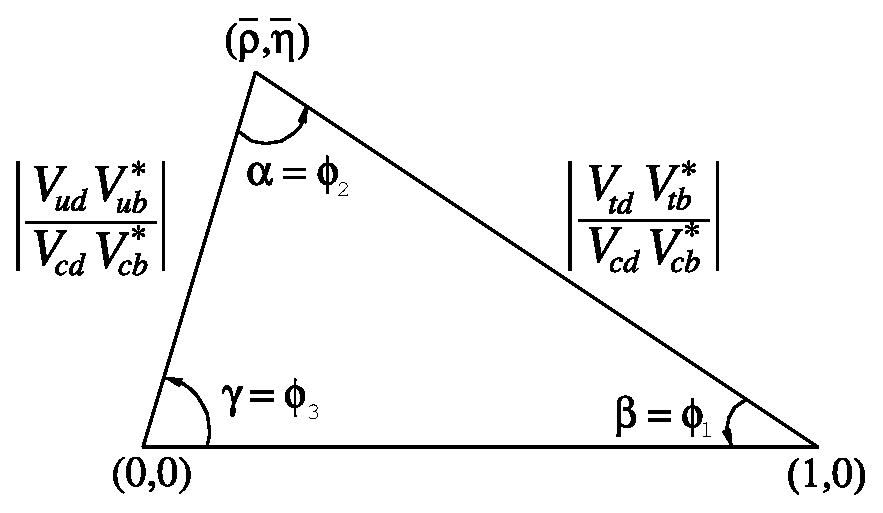
\includegraphics[width=0.5\textwidth]{triangle2.eps}
%\end{figure*}

The area of these triangles are half of the Jarlskog invariant \textit{J}, a quantifier of CP violation, which is defined as $ Im[V_{ij}V_{kl}V^*_{il}V^*_{kj}]$ \cite{jarsklog}. It is independent of phase convention. It is important to emphasize that the Standard Model with its parameters may or may not violate CP. Only after measuring the parameter it is possible to determine the CP non-conservation. \textit{J} vanishes\cite{secondjar} only if mixing angle $\theta_{ij} = 0 , \pi/2$; $\delta =  0 , \pi$; So measurements of \textit{J} allows to verify that the CKM matrix is complex and hence different mixing for quarks and anti-quarks is obtained, providing theoretical grounding for CP violation, one of the Sakharov conditions for the evolution of the universe which we see today, although the standard model CP violation is not big enough to explain the matter dominated universe.

Experimentally the most precise measurement of the CKM matrix\cite{ewconstraint} to-date is 
%\begin{equation}|V_{\rm CKM}| = \begin{pmatrix}0.97427 \pm 0.00015 & 0.22534 \pm 0.00065  &  0.00351\pm \bfrac{0.00015}{0.00014} \cr
%0.22520 \pm 0.00065 &  0.97344 \pm 0.00016 & 0.0412\pm\bfrac{0.0011}{0.0005} \cr
%0.00867 \pm \bfrac{0.00029}{0.00031} & 0.0404 \pm \bfrac{0.0011}{0.0005} &  0.999146 \pm \bfrac{0.000021}{0.000046} \cr \end{pmatrix} .
%\end{equation}

\section{Fully Leptonic $P^{+}\rightarrow l^{+} \nu_{l}$ decays}
This text is based on a summary provided by PDG on Leptonic Decays of Charged Pseudoscalar Mesons.


Purely leptonic decays that proceed by annihilation-type diagrams of pseudoscalar mesons ($P$) are of great interest for flavour physicists because of several reasons as they allow:
\begin{itemize}
\item measurements of the CKM matrix elements,
\item measurements of leptonic decay constants,
\item measurements of the new physics effects.
\end{itemize}



First two types of measurements are possible because the decay rates of $P^{+}\rightarrow l^{+} \nu_{l}$ decays are sensitive to the product of the appropriate CKM matrix element ($V_{q_{1}q_{2}}$ where $q_{1}$ and $q_{2}$ are constituent quarks of the pseudoscalar meson) and decay constant $f_{P}$, related parameter arising from the strong interaction. In more detail, the decay width of fully leptonic decay of a pseudoscalar meson in the Stadard Model to the lowest order can expressed as 

\begin{equation}
%\label{eqn:br} 
\Gamma(P^{+} \rightarrow {l^{+}} \nu_{l})=  
	\frac{G_{F}^{2} m^{}_{P^{+}}  m_{l^{+}}^{2}}{8\pi} 
	\left[1 - \frac{m_{l^{+}}^{2}}{m_{P^{+}}^{2}}\right]^{2}  
	f_{P}^{2} |V_{q_{1}q_{2}}|^{2} 
	,
\label{eqn:dw} 
\end{equation}

where
$G_F$ is the Fermi constant,
$m^{}_{P^{+}}$ and $m_{l^{+}}$ are the pseudoscalar meson and lepton masses, respectively,
$\tau_{P^{+}}$ is the $P^{+}$ lifetime.

So in order to measure CKM matrix amplitude, knowledge of $f_{P}$ must be inferred. $f_{P}$ can be calculated using lattice QCD techniques and together with experimental determination of the decay rates provides provide a way to determine relevant amplitude squared of the relevant CKM matrix element. More conventionally, CKM magnitudes are determined from semileptonic decays, but in this case the sensitivity to different type of current is given. In purely leptonic decays axial-vector flavour-changing currents ($q_{1}\gamma_{\mu}\gamma_{5}q_{2}$) are probed as opposed to vector current ($q_{1}\gamma_{\mu}q_{2}$) in semileptonic case.

Vice versa, assuming unitarity of CKM triangle and experimental determination of relevant $V_{q_{1}q_{2}}$ one can obtain experimental determination of the decay constants and compare it with theoretical prediction.

Last, but not least, is of course the measurement of presence of new physics in these decays. Especially appealing is the presence of new particles which would manifest themselves in the decay rates of heavier pseudoscalars ($D_{(s)}$ or $B$). Example of such new particles include charged Higgs bosons, $H^{\pm}$, coming from so-called Type II of two-Higgs-doublet models \cite{Hou:1992sy}\cite{Akeroyd:2003zr}\cite{Dobrescu:2008er} or leptoquarks\cite{Dobrescu:2008er}. In this case, considering $B^{+}\rightarrow l^{+}\nu$ decay, four-fermion interaction between $W^{\pm}$ and $H^{\pm}$ would modify the SM decay width~\autoref{eqn:dw} to
%remember branching fraction is partial width of total width
%total width  h over liftime so lifetime is always missing from equations 
% see https://www2.ph.ed.ac.uk/~vjm/Lectures/ParticlePhysics2010_files/Particle3-2Nov.pdf this

\begin{equation}
\Gamma(B^{+} \rightarrow {l^{+}} \nu_{l})=  
        \frac{G_{F}^{2} m^{}_{B^{+}}  m_{l^{+}}^{2}}{8\pi} 
        \left[1 - \frac{m_{l^{+}}^{2}}{m_{B^{+}}^{2}}\right]^{2}  
	f_{P}^{2} |V_{ub}|^{2} \,\times\, r_H,
%\Gamma(B^+\to \ell^+\nu_\ell)={G_F^2 m_{B} m_l^2 f_{B}^2\over 8\pi}
%|V_{ub}|^2 \left(1-{m_l^2\over m^2_{B}}\right)^2 \,\times\, r_H
\end{equation}

where
\begin{equation}
	r_H=[1-\tan^2\beta(m^{2}_{B^{+}}/m^{2}_{H^{+}})]^2.
\end{equation}

Here $\tan\beta = \frac{v_{2}}{v_{1}}$, where $v_{i}$ are the vacuum expectation values for the Higgs doublets. In order to have enhancing effect for the rate of $B^{+}\rightarrow l^{+}\nu$ decay (to have $r_{H}>1$), $\tan\beta/H^{\pm}> 0.27 \gev^{-1}$.

Given current tensions arising in flavour physics searches especially concerning lepton non-unversality, ratio of rates between $P\rightarrow\tau\nu$,$P\rightarrow\mu\nu$ and $P\rightarrow e\nu$ should be measured. In the ratios the decay constant $f_{P}$ cancels out making such measurements good tool for lepton universality tests.

As seen in~\autoref{eqn:dw}, purely leptonic final state going through $P\rightarrow W^{*}\rightarrow l \nu$ is supressed by $m^{2}_{l}$, also known as helicity supression. This suppression occurs as a result of angular momentum conservation. In case of $B^{+}\rightarrow l^{+} \nu$, $B^{+}$ is a spin-0 particle and hence its decay products have to have spin 0 combined, or in other words, be anti-aligned. Neutrinos in the SM are always produced left-handed. As the spin of the antilepton and the neutrino should be anti-aligned, antilepton also needs to be left-handed (to have negative helicity). However, the weak current only couples to right-handed antiparticles. Therefore, the antilepton has to be boosted in order to have different helicity. For massless particles such helicity flip is not possible making this decay impossible. The lighter the lepton the larger the velocity and hence higher boost is necessary, making decays to lighter leptons rarer even though they have bigger kinematic phase space available.

%https://www.physicsforums.com/threads/helicity-and-suppression.804600/
The latest experimental measurements for rates of these measurements have been performed by $B$ factories, finding evidence for $B^{+}\rightarrow \tau^{+}\nu$ and first sign of $B^{+}\rightarrow \mu^{+}\nu$ as seen in~\autoref{tab:sum}. These results are to be compared with SM prediction $\mathcal{B}(B^{+}\rightarrow \tau^{+}\nu) = (0.82+0.03-0.02)\times10^{-4}$\cite{Charles:2004jd} which is obtained by using unitarity-constrained $V_{ub}$ value aggregated from other measurements and lattice calculations of $f_{B}$. Quite subtantial statistical as well as systematical errors show the difficulty of this type of measurements. 

\begin{table}[ht]
\begin{center}
\begin{tabular}{ l l l l H c H} \hline
	Process &Experiment & Tag &${\mathcal{B}}$ ($\times$ $10^{-4}$) & Published & Significance ($\sigma$) & {$|V_{ub}|f_{B^+}$ (MeV)} \hfill\\
\hline\\[-2.5ex]
	$B^{+}\rightarrow \tau^{+}\nu$	&Belle~\cite{Adachi:2012mm}&Hadronic&$0.72^{+0.27}_{-0.25}\pm0.11$  & 2013 & 3.0 \\ 
$B^{+}\rightarrow \tau^{+}\nu$	&Belle~\cite{Kronenbitter:2015kls}&Semileptonic&$1.25\pm0.28\pm0.27$ & 2015 & 3.8 \\
$B^{+}\rightarrow \tau^{+}\nu$	&Belle~\cite{Kronenbitter:2015kls}&Average&$0.91 \pm 0.22$ & 2015 & 4.6 \\\hline\\[-2.5ex]
$B^{+}\rightarrow \tau^{+}\nu$	&BaBar~\cite{Lees:2012ju} & Hadronic & $1.83\,^{+0.53}_{-0.49}\pm0.24$ & 2012 & 3.8 \\ 
$B^{+}\rightarrow \tau^{+}\nu$	&BaBar~\cite{Aubert:2009wt} & Semileptonic & $1.7\pm 0.8\pm 0.2$ & 2010 & 2.3\\ 
$B^{+}\rightarrow \tau^{+}\nu$	&BaBar~\cite{Lees:2012ju} & Average & $1.79 \pm 0.48$ & 2012 & - & $1.01\pm 0.14$  \\ \hline
$B^{+}\rightarrow \mu^{+}\nu$ & Belle~\cite{Sibidanov:2017vph} & Untagged& $(6.46\pm2.22\pm 1.60)\times 10^{-3}$ & 2017 & 2.4 &\\
%        & Our average & &$1.06\pm0.20$&$0.77\pm0.07$ & & \\
\hline
\end{tabular}
\end{center}
\caption{Experimental summary of searches for $B^{+}\rightarrow l^{+}\nu$.}
\label{tab:sum}
\end{table}


With helicity supressed rates and very limited signature in the detector (one chaged track for muons and electron, more charged tracks for taus, but also more missing energy depending on the reconstruction channel) searching for such decays is still very challenging. In order to make measurements of the same kind (CKM precision measurements, decay constants measurements, new physics searches), fully leptonic decays but with photons can be considered.   

\section{Fully Leptonic $B^{+}\rightarrow l^{+} \nu_{l} \gamma$ decays}
The helicity suppression can be lifted by considering the decay with an additional photon radiated from the $B^{+}$ meson, at the cost of the electromagnetic suppression with coupling constant $\alpha_{em}$. Consequently, the branching fraction for radiative decays can be comparable or even larger than the corresponding fraction for purely leptonic decays. It has been shown that $R^{\mu}_{B}=\frac{\Gamma(B\rightarrow \mu \nu \gamma)}{\Gamma(B\rightarrow \mu \nu)}\approx(1-20)$ making $\mathcal{B}(B\rightarrow \mu \nu \gamma)\approx(10^{-7}-10^{-6})$ \cite{Burdman:1994ip}.

As compared to photonless decays the amplitude of the decay will have contribution from both axial-vector weak current as well as vector current.
The differential decay width with $\frac{1}{m_{b}}$ and radiative corrections
at next-to-leading logarithmic order calculated in\cite{Beneke:2011nf} is given by the following formula:
\begin{equation}
\frac{d\Gamma}{dE_{\gamma}} = \frac{\alpha_{em}G^{2}_{F}|V_{ub}|^{2}}{48 \pi^{2}}m_{B}^{4}(1 - x_{\gamma})x_{\gamma}^{3}[F_A^{2} + F_V^{2}]
\end{equation}
 where $x_{\gamma} = 2E_{\gamma}/m_{B}$, $F_A$ is axial form factor and $F_V$  is vector form factor defined as
\begin{equation}
F_{V}(E_{\gamma}) = \frac{Q_{u}m_{B}f_{B}}{2E_{\gamma}\lambda_{B}(\mu)} R(E_{\gamma}, \mu) + [\xi(E_\gamma) +  \frac{Q_{u}m_{B}f_{B}}{(2E_{\gamma})^{2}} + \frac{Q_{b}m_{B}f_{B}}{2E_{\gamma}m_{b}}],
\end{equation}

\begin{equation}
F_{A}(E_{\gamma}) = \frac{Q_{u}m_{B}f_{B}}{2E_{\gamma}\lambda_{B}(\mu)} R(E_{\gamma}, \mu) + [\xi(E_\gamma) -  \frac{Q_{u}m_{B}f_{B}}{(2E_{\gamma})^{2}} - \frac{Q_{b}m_{B}f_{B}}{2E_{\gamma}m_{b}} + \frac{Q_{l}f_{B}}{E_{\gamma}}].
\end{equation}
Here $Q_{l},Q_{u},Q_{b}$ are the charges of the lepton, up quark, and
bottom quark, respectively, $f_{B}$ is the decay constant for
the B meson, and $R(E_{\gamma}, \mu)$ is a radiative correction
calculated at the energy scale $\mu$ %that equals one at tree level.
and $m_{b}$ is the mass of $b$ quark.

The term not in squared brackets represents the leading-power contribution in the heavy-quark expansion. Note that this term
is the same for the vector and axial form factor. The terms in square brackets are $\frac{1}{m_{b}}$ power corrections relative to the leading term. Further corrections have been discussed in~\cite{Wang:2016beq}.



Recent measurement of the radiative $B^{+} \rightarrow l^{+} \nu_{l} \gamma$, where $l^{+}$ is either $e^{+}$ or $\mu^{+}$ was performed by Belle using hadronic tagging on their full data sample\cite{Heller:2015vvm}.The search yielded $\mathcal{B}(B^{+}\rightarrow \mu^{+} \nu_\mu \gamma) < 3.4\times 10^{-6}$ \cite{Heller:2015vvm}.



\section{Fully Leptonic $B^{+}\rightarrow l^{+} l^{-} l^{+} \nu_{l} $ decays}


In LHCb, the most optimal approach due to the detector capabilities is to measure this kind of decay by decaying the photon into pair of muons, see~\autoref{fig:myfeyn}(a). If the naive expectation of only taking into account photon conversion into two muons is adopted, then the expected branching fraction for this analysis is $\mathcal{B}(B^{+}\rightarrow \mu^{+} \mu^{-} \mu^{+} \nu_{\mu}) \approx 10^{-8}$. However, such estimate is not correct because there are other contributions to the total decay rate as shown in the first theoretical prediction for $\mathcal{B}(B^{+}\rightarrow \mu^{+} \mu^{-} \mu^{+} \nu_{\mu})$ in \cite{Danilina:2017bcn} based on Vector Meson Dominance (VMD) model. This theoretical prediction yields $\mathcal{B}(B^{+} \rightarrow \mu^{+} \mu^{-} \mu^{+} \nu_{\mu}) \approx 1\times 10^{-7}$ and the rest of this section is a short summary of this publication.

VMD model was formulated to describe the interaction between photon and hadrons before quantum chromodynamics was formulated. It is an approximative model where photon is treated to be made of both purely electromagnetic component and vector meson component. This idea originates in the fact that both photon and vector mesons have the same quantum numbers $J^{PC} = 1^{-\ -}$ and if two particles have the same quantum numbers then they mix (the state which commutes with the Hamiltonian is a superposition of all such states). Therefore there is mixing between $\gamma$ and vector mesons.

As mentioned previously, there are different contributions to the amplitude of the $\mathcal{B}(B^{+}\rightarrow \mu^{+} \mu^{-} \mu^{+} \nu)$. Using VMD model, it is no suprising that the biggest contribution arises the photon emission from the valence $u$-quark of the $B$ meson. In this case, contribution from $\rho(770)$ and $\omega(782)$ resonances are included in the calculation. Secondly, contribution of photon emission from the $b$-quark is studied, effectively creating excited $B^{+}$, $B^{+*}$ intermediate resonance state. Thirdly, photon can be emitted from the final-state lepton, process known as Brehmstrahlung. All these different contributions to the decay amplitude are shown in \autoref{fig:myfeyn}. To obtain the total amplitude, sum of the matrix elements of the three contributions is calculated in the limit where $m_{l}$ is set to zero.


\begin{figure}[ht]
\centering
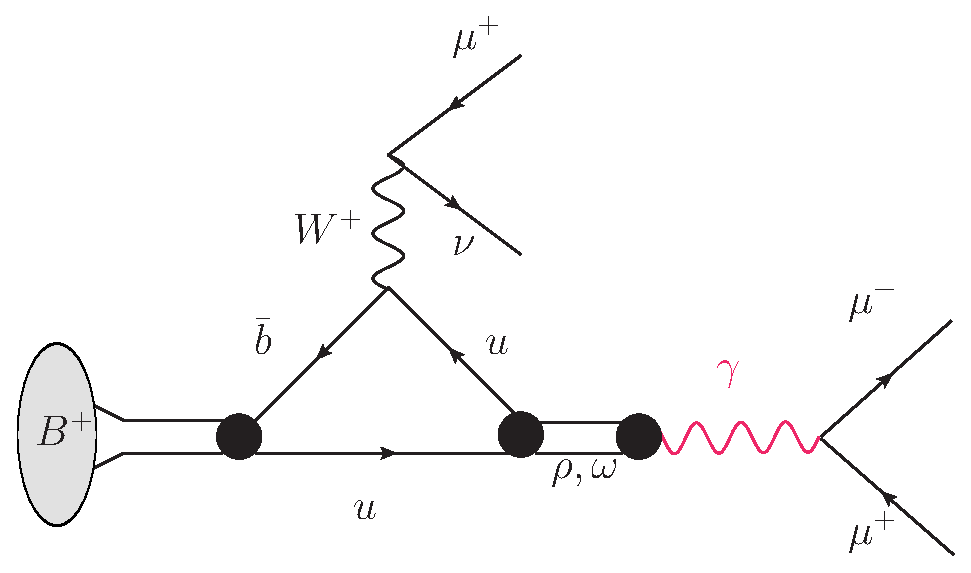
\includegraphics[scale=0.5]{theory/nik_1figure}\put(-30,133){(a)}
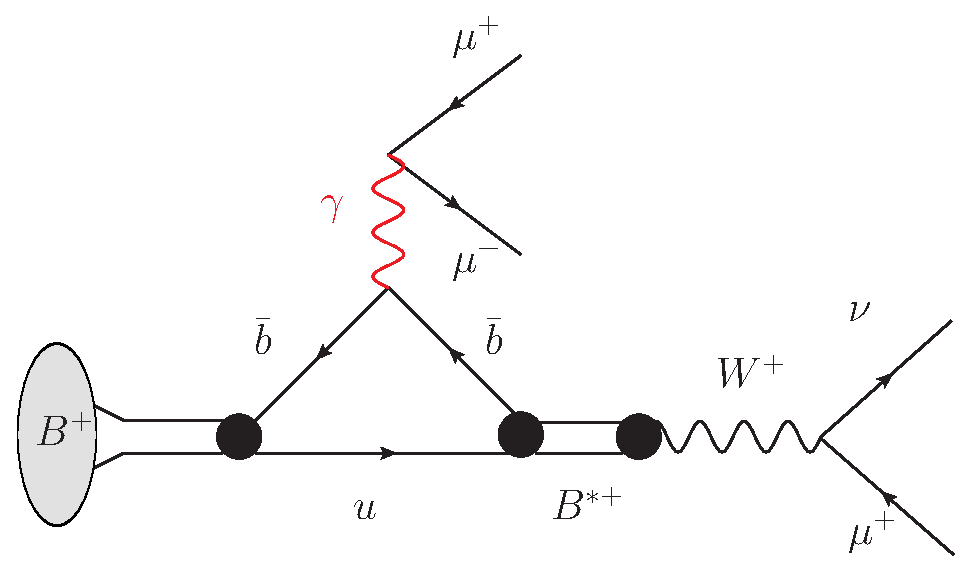
\includegraphics[scale=0.5]{theory/nik_2figure}\put(-30,133){(b)}
\newline
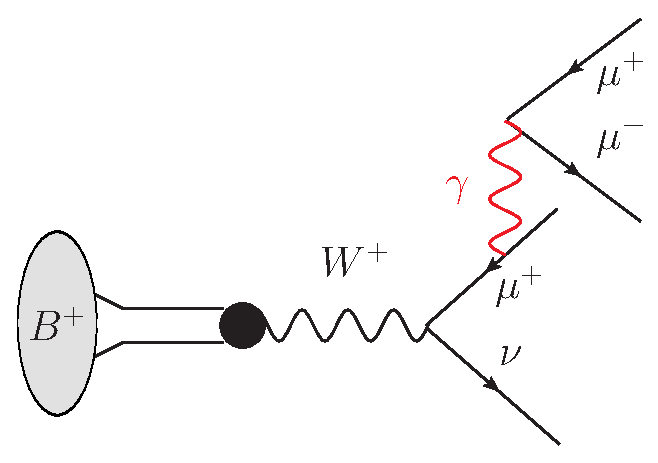
\includegraphics[scale=0.55]{theory/nik_3figure}\put(-30,133){(c)}
\centering
	\caption{(a) Annihilation diagram where the initial $u$-quark state radiates off a virtual photon which decays into a pair of muons and the $W^{+}$ decays into a muon and muon neutrino. Most of the contribution to the rate comes from hadronic contribution to the photon. (b) Photon emission from $b$-quark and (c) finally emission from the final state muon.}
\label{fig:myfeyn}
\end{figure}


In this publication the amplitude of $\mathcal{B}(B^{+}\rightarrow \mu^{+} \mu^{-} \mu^{+} \nu)$ is estimated by calculating $\mathcal{B}(B^{+}\rightarrow \mu^{+} \mu^{-} e^{+} \nu)$ amplitude first and then adding an negative interference term that arises due to the identical fermions in the final state doubling the number of possible diagrams. The numerical calculation yields $\mathcal{B}(B^{+}\rightarrow \mu^{+} \mu^{-} e^{+} \nu) \approx 1.3 \times 10^{-7}$ and $\mathcal{B}(B^{+}\rightarrow \mu^{+} \mu^{-} \mu^{+} \nu) \approx 1.0 \times 10^{-7}$. 

\section{\Bmumumu decay model}
As the search for \Bmumumu decay is first of its kind, simulation that describes this type of decay was not available. 

For any decay, it is possible to use phase space model, \textit{PHSP}, which only takes into account the kinematic constraints of the decay without taking into account any input from theoretical considerations as the matrix element is constant. This is not satisfactory for decays where there are intermediate virtual photons or vector mesons resonances.

Following decay model is developped to take into the account more correct behaviour of the leading order contribution to the decay shown in~\autoref{fig:myfeyn}(a). The decay proceeds through a virtual $W$ decaying to $\mu^{+} \nu$ and a virtual photon with vector resonance decaying to a muon pair. This has similar structure to $\B^{+} \rightarrow (K^{*+}) \mu^{+} \mu^{-}$ decay, where the $K^{*+}$ can take the role of the virtual $W$ decay. By using the \textit{BTOSLLBALL} model\cite{Ali:1999mm}, traditionally used for $B^{+} \rightarrow (K^{*+}) l^{+} l^{-}$ decays, but modifying properties of the $K^{*+}$ to those of virtual $W$ (having mass of 0.1 \gevcc and width 50 \gev), it is possible to obtain good approximation to the correct features of the decay . This is shown in~\autoref{fig:mcgeneration}, where there is a characteristic photon pole for low $q(\mu^{+},\mu^{-})$, invariant mass of the opposite muon pair, and flat distribution for $K^{*}(\mu^{+}, \nu_{\mu}) $, invariant mass of the muon and neutrino pair. This decay model will be further referred to as SALLY's model. 


%\mybox{Sally: move it to theory and check ulrik's comment} In order to produce simulation with a decay model which is more representative of the spin structure involved, the following strategy is adapted. In this simulation approach, the decay proceeds as follows: \Bpm decays into \Wpm and a pair of opposite sign muons and then \Wp is decayed to $\mu^{+} \nu$. \textit{BTOSLLBALL} model\cite{Ali:1999mm}, traditionally used for $\B \rightarrow (K,K^{*}) l^{+} l^{-}$ decay, with the form factor calculations can be used to simulate $\Bpm \rightarrow \Wpm l^{+} l^{-}$ decay. After that, \Wp is decayed to $\mu^{+} \nu$ using \textit{PHSP}. For semileptonic $b \rightarrow s l^{+} l^{-}$ transitions, there is a characteristic photon pole for low $q(\mu^{+},\mu^{-})$, invariant mass of the opposite muon pair, and flat distribution for $K^{*}(\mu^{+}, \nu_{\mu}) $, invariant mass of the muon and neutrino pair. In order to achieve this, a new pseudo-particle is introduced to EVTGEN with specific properties, $K^{*}(\mu^{+}, \nu_{\mu})$, and the best output can be seen to be for a particle $K^{*}(\mu^{+}, \nu_{\mu})$ with mass to be set to $0.1 \text{GeV/c}^{2}$, and width, corresponding to $\tau= 1.3\times10^{-17}$ nanoseconds as can be seen in \autoref{fig:mcgeneration}. This procedure was also applied for the charge conjugate case. This model is denoted as \textit{INSP} and is used as default in mass fits and efficiency calculations.

\begin{figure}[h!]
\centering
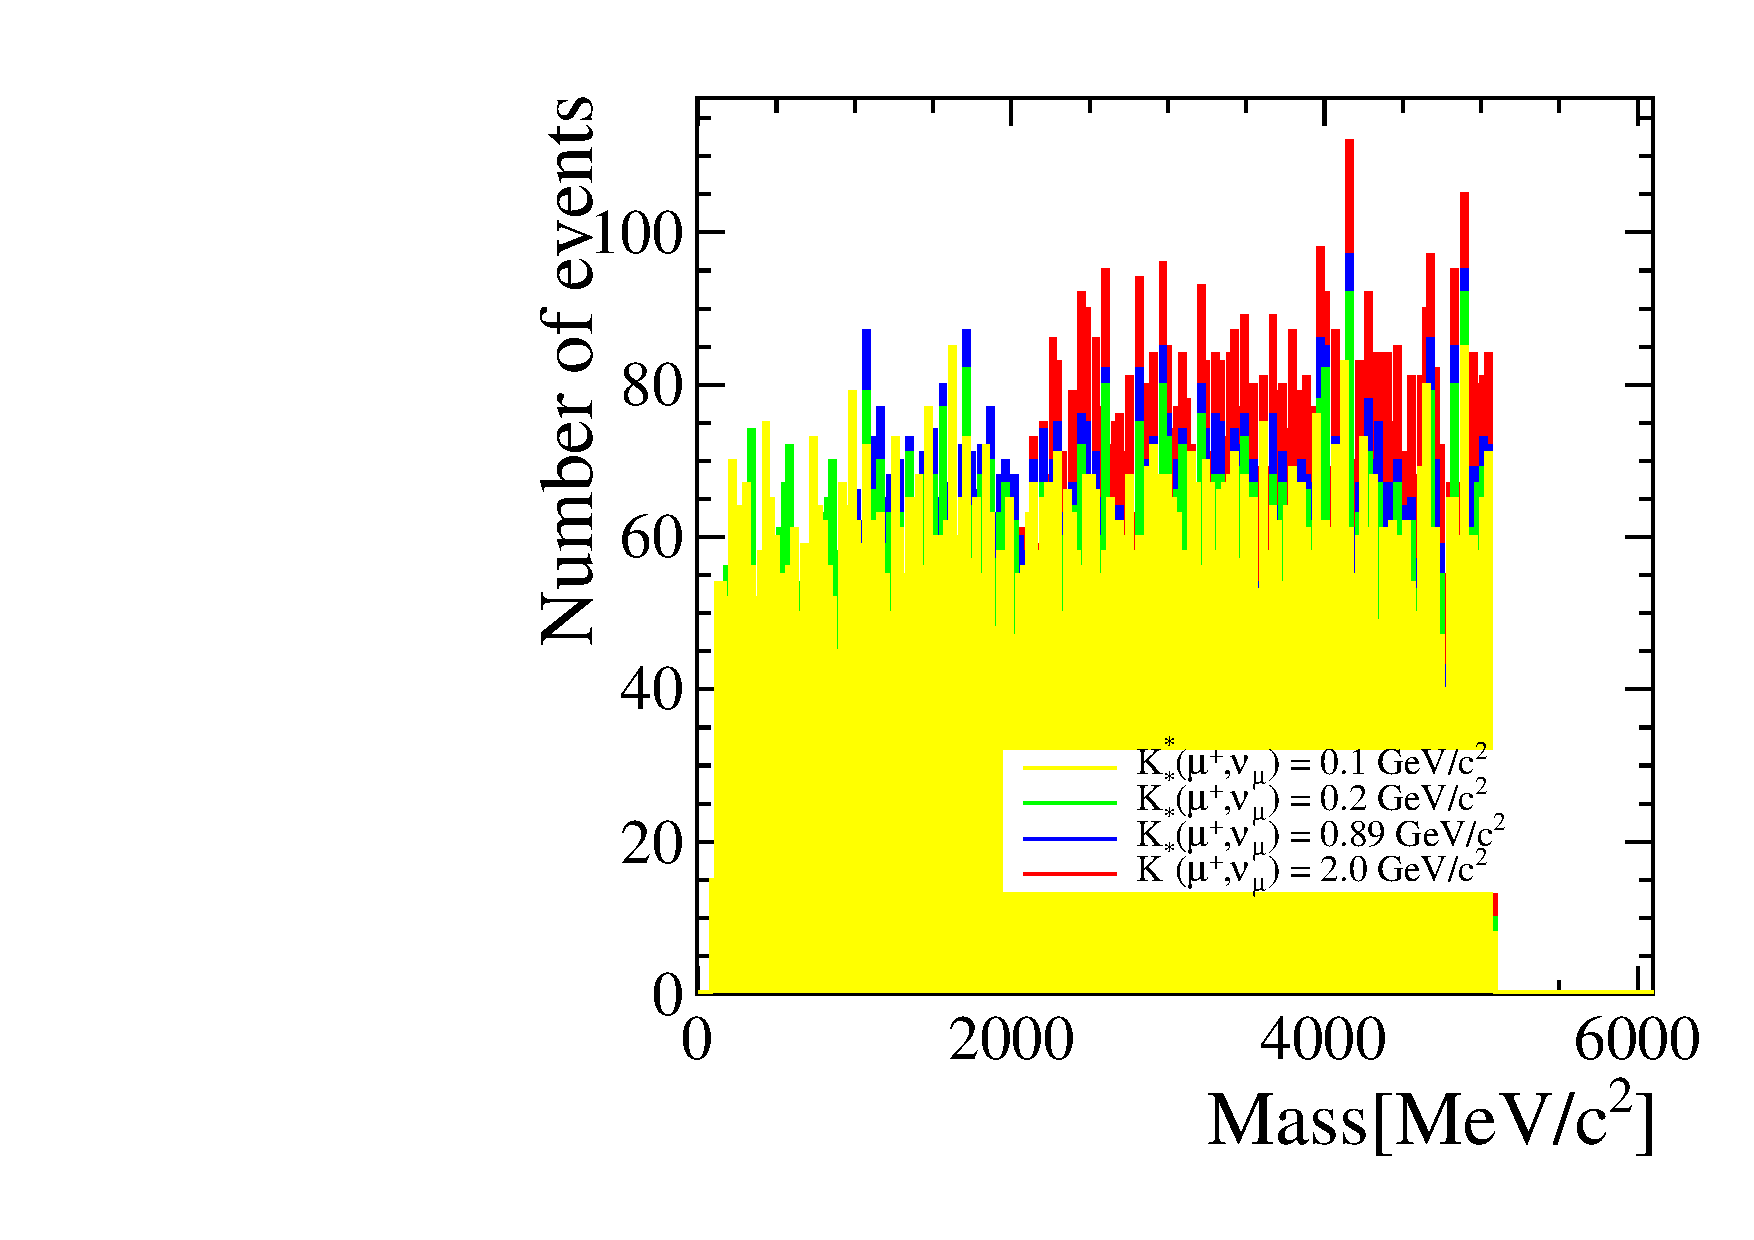
\includegraphics[width=0.5\linewidth]{./sel/reporttry_new}\put(-70,133){(a)}
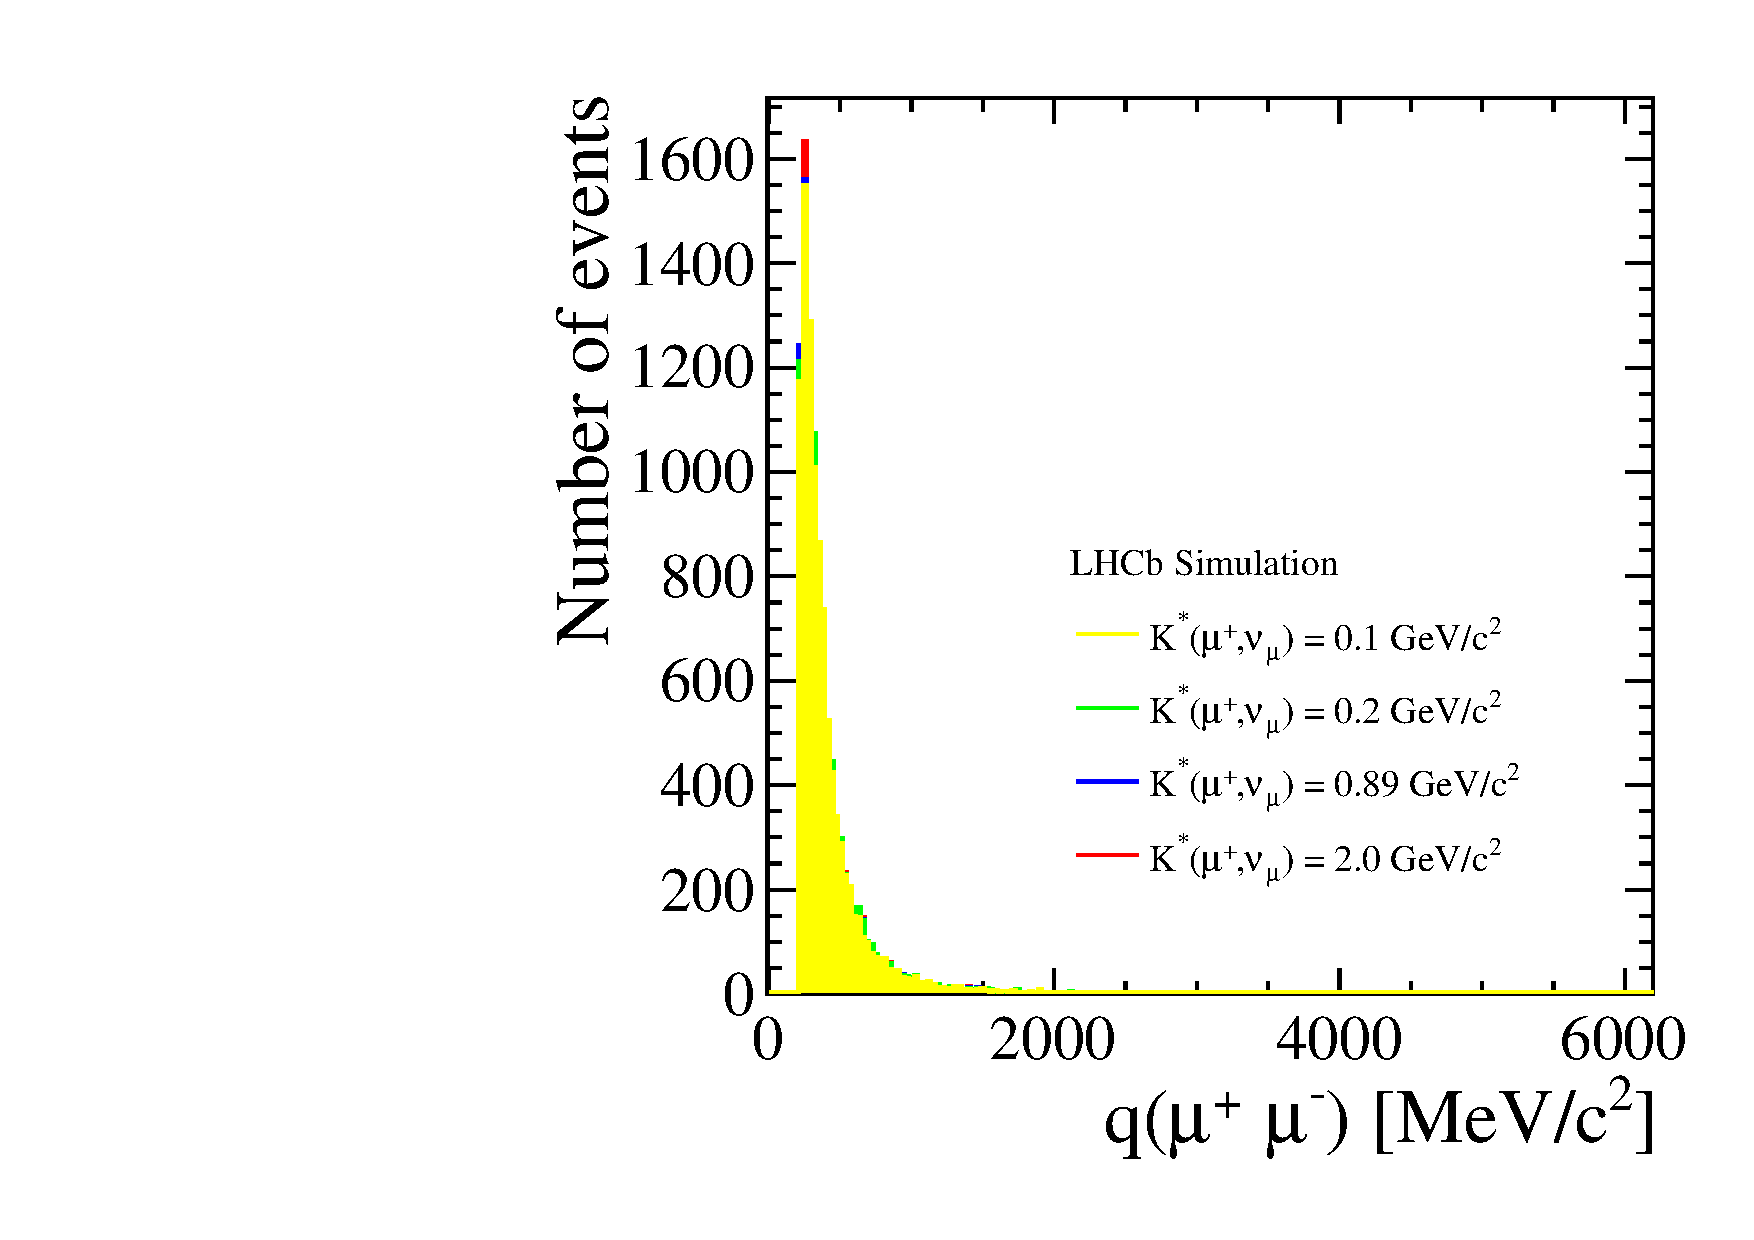
\includegraphics[width=0.5\linewidth]{./sel/reporttrialqpres_new}\put(-50,133){(b)}
\caption{Distributions for signal MC in using Pythia 6.4 \cite{pythia6} conditions. (a) $K^{*}(\mu^{+}, \nu_{\mu})$ (b) $q(\mu^{+},\mu^{-})$ distributions under different $K^{*}$ mass hypotheses. The most flat distribution in $K^{*}(\mu^{+}, \nu_{\mu})$ is plotted in yellow.}
\label{fig:mcgeneration}
%\vspace*{-1.0cm}
\end{figure}



